\documentclass[a4paper,12pt]{article}


\usepackage{mathtext}
\usepackage[T2A]{fontenc}
\usepackage[utf8]{inputenc}
\usepackage[russian]{babel}
\usepackage{amsmath}
\usepackage{amsfonts}
\usepackage{amssymb}
\usepackage{graphicx}
\usepackage{nameref}
\usepackage{subcaption}
\usepackage[margin=1.5pt]{geometry}
\usepackage{float}
\usepackage{latexsym}
\usepackage{stmaryrd}
\usepackage{hyperref}
\usepackage{listings}
\usepackage{xcolor}
\usepackage{tabularx}


\geometry{left=2cm, right=2cm, top=2cm, bottom=2cm}

\begin{document}

\definecolor{codegreen}{rgb}{0,0.6,0}
\definecolor{codegray}{rgb}{0.5,0.5,0.5}
\definecolor{codepurple}{rgb}{0.58,0,0.82}
\definecolor{backcolour}{rgb}{1,1,1}

\lstdefinestyle{pythonStyle}{
    backgroundcolor=\color{backcolour},
    commentstyle=\color{codegreen},
    keywordstyle=\color{red},
    numberstyle=\tiny\color{codegray},
    stringstyle=\color{codepurple},
    basicstyle=\ttfamily\footnotesize,
    breakatwhitespace=false,
    breaklines=true,
    captionpos=b,
    keepspaces=true,
    numbers=left,
    numbersep=5pt,
    showspaces=false,
    showstringspaces=false,
    showtabs=false,
    tabsize=2
}
\lstset{style=pythonStyle}

\pagestyle{empty}

\begin{center}
\textbf{МИНОБРНАУКИ РОССИИ}\\
ФЕДЕРАЛЬНОЕ ГОСУДАРСТВЕННОЕ БЮДЖЕТНОЕ \\
ОБРАЗОВАТЕЛЬНОЕ УЧРЕЖДЕНИЕ ВЫСШЕГО ОБРАЗОВАНИЯ \\
ВОРОНЕЖСКИЙ ГОСУДАРСТВЕННЫЙ УНИВЕРСИТЕТ \\
Факультет прикладной математики, информатики и механики\\
Кафедра вычислительной математики и прикладных информационных технологий
\end{center}

\vspace{2cm}
\begin{center}
\textbf{ЛАБОРАТОРНАЯ РАБОТА №3}\\
\textbf{ЧИСЛЕННОЕ РЕШЕНИЕ СТАЦИОНАРНОГО УРАВНЕНИЯ ШРЁДИНГЕРА: РАСЧЁТ ОСНОВНОГО КВАНТОВОГО СОСТОЯНИЯ ЧАСТИЦЫ В ОДНОМЕРНОЙ ПОТЕНЦИАЛЬНОЙ ЯМЕ С БЕСКОНЕЧНЫМИ СТЕНКАМИ С ИСПОЛЬЗОВАНИЕМ РАЗЛОЖЕНИЯ ИСКОМОЙ ВОЛНОВОЙ ФУНКЦИИ ПО БАЗИСУ}
\end{center}

\vspace{3cm}
\begin{flushright}
\begin{tabular}{l l}
\textbf{Направление:} & 01.04.02 \textendash{} Прикладная математика и информатика \\
\textbf{Выполнил:} & студент 11 группы 2 курса магистратуры \\
& Крутько А.С. \\
\textbf{Преподаватель:} & доктор физ.-мат. наук, профессор Тимошенко Ю.К.
\end{tabular}
\end{flushright}

\vspace{3cm}
\begin{center}
Воронеж 2024
\end{center}

\newpage
\tableofcontents
\pagestyle{plain}
\setcounter{page}{2}

\newpage
\section{Цели и задачи работы}\label{sec:goals}
\subsection{Цель работы.}\label{subsec:-.}
Целями лабораторной работы являются практическое освоение информации, полученной при изучении курса <<Компьютерное моделирование в математической физике>> по теме <<Численное решение стационарного уравнения Шрёдингера>>, а также развитие алгоритмического мышления и приобретение опыта использования знаний и навыков по математике, численным методам и программированию для решения прикладных задач физико-технического характера.

\subsection{Задачи работы:}\label{subsec:-:}

\textbf{Проблема:} электрон находится в одномерной потенциальной яме с бесконечными стенками $U(x)$:
\[
v(x) =
    \begin{cases}
        L_5(x), & x \in (-L, L), \\
        \infty, & x \notin (-L, L),
    \end{cases}
\]
Где $U(x) = v(x)*V_0$, $V_0 = 25$ \text{эВ}, $L = 3$ \AA, $L_n(x)$ -- полином Ляггера, $n = 5$.

\begin{enumerate}
    \item Рассчитать энергию и волновую функцию основного квантового состояния путем разложения искомой волновой функции по базису.
          Использовать в качестве базисного набора - волновые функции частицы в одномерной прямоугольной яме с бесконечными стенками.
    \item Вычислить для этих состояний квантовомеханические средние $\langle p(x) \rangle$ и $ \langle p(x^2) \rangle $.
\end{enumerate}

\newpage
\section{Одномерное стационарное уравнение Шрёдингера. Математический формализм. Общие свойства решений}\label{sec:-}
Одномерное стационарное уравнение Шрёдингера~\cite{tim_shrod}:
\begin{equation}
    \hat{H}\psi(x) = E\psi(x),
    \label{eq:oneDimShrodingerEq}
\end{equation}
где $\hat{H}$ \textendash{} оператор Гамильтона, $E$ \textendash{} собственные значения энергии, $\psi(x)$ \textendash{} волновая функция.

С математической точки зрения оно представляет собой задачу определения собственных значений $E$ и собственных функций $\psi$ оператора Гамильтона $\hat{H}$.
Для частицы с массой $m$, находящейся в потенциальном поле $U(x)$, оператор Гамильтона имеет вид
\begin{equation}
    \hat{H} = \hat{T}+ U(x),
    \label{eq:gamilton_op}
\end{equation}
где оператор кинетической энергии
\begin{equation}
    \hat{T} =-\frac{\hslash^2}{2m}\frac{d^2}{dx^2},
    \label{eq:gamilton_kinetic_e_op}
\end{equation}
а $\hslash$ --- постоянная Планка.
Собственное значение оператора Гамильтона имеет смысл энергии соответствующей изолированной квантовой системы.
Собственные функции называются волновыми функциями.
Волновая функция однозначна и непрерывна во всём пространстве.
Непрерывность волновой функции и её первой производной сохраняется и при обращении $U(x)$ в $\infty$ некоторой области пространства.
В такую область частица вообще не может проникнуть, то есть в этой области, а также на её границе $\psi(x)=0$.

Оценим нижнюю границу энергетического спектра.
Пусть минимальное значение потенциальной функции равно $U_{\min}$.
Очевидно, что $\langle T \rangle \geq 0$ и $\langle U \rangle \geq U_{\min}$.
Потому из уравнения~\eqref{eq:oneDimShrodingerEq} следует, что:
\begin{equation}
    E =\langle H\rangle = \int_{-\infty}^{+\infty} \psi^\star(x)\hat{H}\psi(x) \,dx =\langle T\rangle +\langle U\rangle > U_{\min}.
\label{eq:e_h_integral}
\end{equation}
то есть, энергии всех состояний > $U_{min}$.

Особый практический интерес представляет случай, когда
\begin{equation}
    \lim_{x\to\infty} U(x) = 0.
\label{eq:limit_pot_inf}
\end{equation}

Потенциал такого типа называется также потенциальной ямой.
Для данной $U(x)$ свойства решений уравнения Шрёдингера зависят от знака собственного значения $E$.
Если $E < 0$.
Частица с отрицательной энергией совершает финитное движение.
Оператор Гамильтона имеет дискретный спектр, то есть собственные значения и соответствующие собственные функции можно снабдить номерами.
При~$E < 0$ уравнение~\eqref{eq:oneDimShrodingerEq} приобретает вид\cite{tim_shrod}:

\begin{equation}
    \hat{H}\psi_k(x) = E_k\psi_k(x).
    \label{eq:shrodinger_eq_e_less_0}
\end{equation}

Квантовое состояние, обладающее наименьшей энергией, называется основным.
Остальные состояния называют возбужденными состояниями.
В силу линейности стационарного уравнения Шрёдингера, волновые функции математически определены с точностью до постоянного множителя.
Однако, из физических соображений, волновые функции должны быть нормированы следующим образом:

\begin{equation}
    \int_{-\infty}^{+\infty} |\psi_k(x)|^2, dx = 1.
    \label{eq:wave_func_normalization}
\end{equation}

В дальнейшем будет рассматриваться только дискретный спектр.
При этом необходимо пользоваться \textbf{осцилляционной теоремой}.

\textbf{Осцилляционная теорема.}
Упорядочим собственные значения оператора Гамильтона в порядке возрастания, нумеруя энергию основного состояния индексом "0": $E_0$, $E_1$, $E_2$ \dots, $E_k$,\dots.
Тогда волновая функция $\psi_k(x)$ будет иметь $k$ узлов (то есть, пересечений с осью абсцисс).
Исключения: области, в которых потенциальная функция бесконечна.

\newpage

\section{Прямой вариационный метод. Алгоритм}\label{sec:solve_method}
К числу приближенных методов вычисления собственных значений и собственных функций оператора Гамильтона относится метод стационарных возмущений Релея-Шрёдингера\cite{tim_pertrubations}, который мы далее будем просто называть «методом» или «теорией возмущений».


В рамках этого теоретического подхода предполагается, что оператор Гамильтона, чьи собственные значения и собственные функции требуется определить, может быть представлен в виде:
\begin{equation}
    \label{eq:gamilton_op}
    \hat{H} = \hat{H}^0 + \hat{V}
\end{equation}
где $\hat{H}^0$ -- гамильтониан идеализированной задачи, решение которой можно найти либо аналитически, либо относительно простым численным путем;~\hat{V} -- называется оператором возмущения или просто возмущением.


Оператором возмущения может быть либо часть гамильтониана, которая не учитывалась в идеализированной задаче, либо потенциальная энергия, связанная с наличием внешнего воздействия.


Идеализированную систему, которую описывает гамильтониан~$\hat{H}^0$, называют «невозмущенной» системой, а систему с гамильтонианом~$\hat{H}$ -- «возмущенной» системой.
В рамках теории возмущений удаётся получить формулы, определяющие энергии и волновые функции стационарных состояний через известные значения энергий~$E_n^{(0)}$ и волновых функций~$\Psi_n{(0)}$ невозмущенной системы.


Стационарные уравнения Шрёдингера для невозмущенной ив возмущенной систем~\cite{tim_pertrubations} имеют вид:
\begin{equation}
\label{eq:stationary_eq_shrod0}
\hat{H}^{(0)}\Psi_n^{(0)}(x)=E_n^{(0)}\Psi_n^{(0)};
\end{equation}

\begin{equation}
\label{eq:stationary_eq_shrod}
\hat{H}\Psi_n(x)=E_n\Psi_n(x).
\end{equation}


В теории возмущений решения уравнения~\eqref{eq:stationary_eq_shrod} ищутся в виде рядов:


\begin{equation}
\label{eq:E_Psi_n_sum}
\begin{split}
    &E_n=E_n^{(0)} + E_n^{(1)} + E_n^{(2)} +\dots =\sum_{k=0}^{\infty}E_n^{(k)},\\
    &\Psi_n(x)=\Psi_n^{(0)}(x) + \Psi_n^{(1)}(x) + \Psi_n^{(2)}(x) +\dots =\sum_{k=0}^{\infty}\Psi_n^{(k)}(x),
\end{split}
\end{equation}
где~$E_n^{k}$, $\Psi_n^{(k)}$ -- величины $k$-го порядка малости по возмущению $\hat{V}$, называемые $k$-ми поправками или поправками $k$-го порядка.
Первые слагаемые рядов~\eqref{eq:E_Psi_n_sum} определяются следующими формулами:
\begin{equation}
\begin{split}
    \label{eq:EPsi_nk_first}
    &E_n^{(1)}=V_{nn}, \\
    &E_n^{(2)}=\sum_m^{\prime}{\frac{|V_{mn}|^2}{E_n^{(0)}-E_m^{(0)})}}, \\
    &\Psi_n^{(0)}(x)=\sum_m^{\prime}{\frac{V_{mn}}{E_n^{(0)}-E_m^{(0)}}}\Psi_m^{0}(x),
\end{split}
\end{equation}
где
\begin{equation}
    \label{eq:v_mn}
    V_{mn}\equiv \langle{m|V|n}\rangle=\int_{\Omega}{\Psi_m^{(0)\star}(x)\hat{V}\Psi_n^{(0)}(x)dx.}
\end{equation}


Штрих над знаком суммы означает пропуск слагаемого с $m=n: \sum_m^{\prime}\equiv \sum_{m\neq n}$.
Очевидно, что ряды в~\eqref{eq:E_Psi_n_sum} сходятся, если выполняется равенство

\begin{equation}
    \label{eq:eq_for_conj}
    |V_{mn}|\ll|E_n^{(0)}-E_m^{(0)}|.
\end{equation}


Во многих случаях для решения задачи достаточно ограничиться вычислением энергии с учетом поправок до второго порядка включительно волновой функции с учетом поправок первого порядка\cite{tim_pertrubations}:

\begin{equation}
\label{eq:first_order_e_psi}
\begin{split}
    &E_n = E_n^{(0)}+V_{nn}+\sum_m^{\prime}{\frac{|V_{mn}|^2}{E_n^{(0)}-E_m^{(0)}}}, \\
    &\Psi_n(x)=\Psi_n^{(0)}(x)+\sum_m^{\prime}{\frac{V_{mn}}{E_n^{(0)}-E_m^{(0)}}\Psi_m^{(0)}(x)}.
\end{split}
\end{equation}


При вычислении второй поправки к энергии и первой поправки к волновой функции основного состояния возмущенной системы бесконечные суммы в~\eqref{eq:E_Psi_n_sum} заменяются конечными.
Для оценки корректного численного значения надо выполнить несколько расчетов соответствующей суммы для монотонно возрастающих величин.
Если увеличение верхнего предела суммы, начиная с некоторого значения, не приводит к заметным изменениям суммы, то задача оценки значения верхнего значения суммы решена.

\newpage

\section{Программная реализация алгоритма}\label{sec:--}
В~\nameref{sec:extras} представлена программа на языке Python 3.12\cite{python},
реализованная в среде разработки PyCharm Community Edition 2024.3.1,
численного решения одномерного стационарного уравнения Шрёдингера для электрона в одномерной потенциальной яме.
Программа реализует алгоритм теории возмущений,
позволяющий находить собственные значения и соответствующие им волновые функции.
Потенциальная функция (невозмущенная система) и параметры для нее соответствуют постановке задачи из первой главы.
Энергия и длина ямы были переведены в атомные единицы Хартри (строки~\textbf{Х}--\textbf{Х}).


В строках~\textbf{Х}--\textbf{Х} определена потенциальная функция.


В строках~\textbf{Х}--\textbf{Х} реализована функция вычисляющая базисную волновую функцию $k$-го состояния.


В строках~\textbf{Х}--\textbf{Х} реализована функция, вычисляющая матричный элемент по формулам (\ref{eq:gamilton_op_components}, ~\ref{eq:gamilton_kinetic_e}, ~\ref{eq:gamilton_pot_e}), функция реализованная в строках~\textbf{Х}--\textbf{Х} является вспомогательной и вычисляет вторую производную для заданной функции.


В строках~\textbf{Х}--\textbf{Х} реализовано построение матрицы Гамильтона.


В строках~\textbf{Х}--\textbf{Х} реализована функция вычисляющая собственные значения и собственные вектора заданной матрицы.


В строках~\textbf{Х}--\textbf{Х} реализована функция вычисляющая волновую функцию по формуле~\eqref{eq:ortonorm_basis_func}


В строках~\textbf{Х}--\textbf{Х} реализованы функции вычисляющие квантовомеханические средние $\langle p(x) \rangle$ и $\langle p(x^2) \rangle$.


В строках~\textbf{Х}--\textbf{Х} реализована функция выводящая графики волновых функций.


В строках~\textbf{Х}--\textbf{Х} задаются размерность сетки и матрицы Гамильтона.


В строках~\textbf{Х}--\textbf{Х} вычисляются энергии и волновые функции и производится запись результата вычислений в файл.

\newpage

\section{Результаты численных экспериментов}\label{sec:results}
Ниже продемонстрированы результаты работы программного кода написанного на Python.


Волновая функция основного состояния, полученного методом Ритца и её плотность представлены на Рис.~\ref{fig:State0PB}

\graphicspath{{../python_results}}

\begin{figure}[h]
\centering
    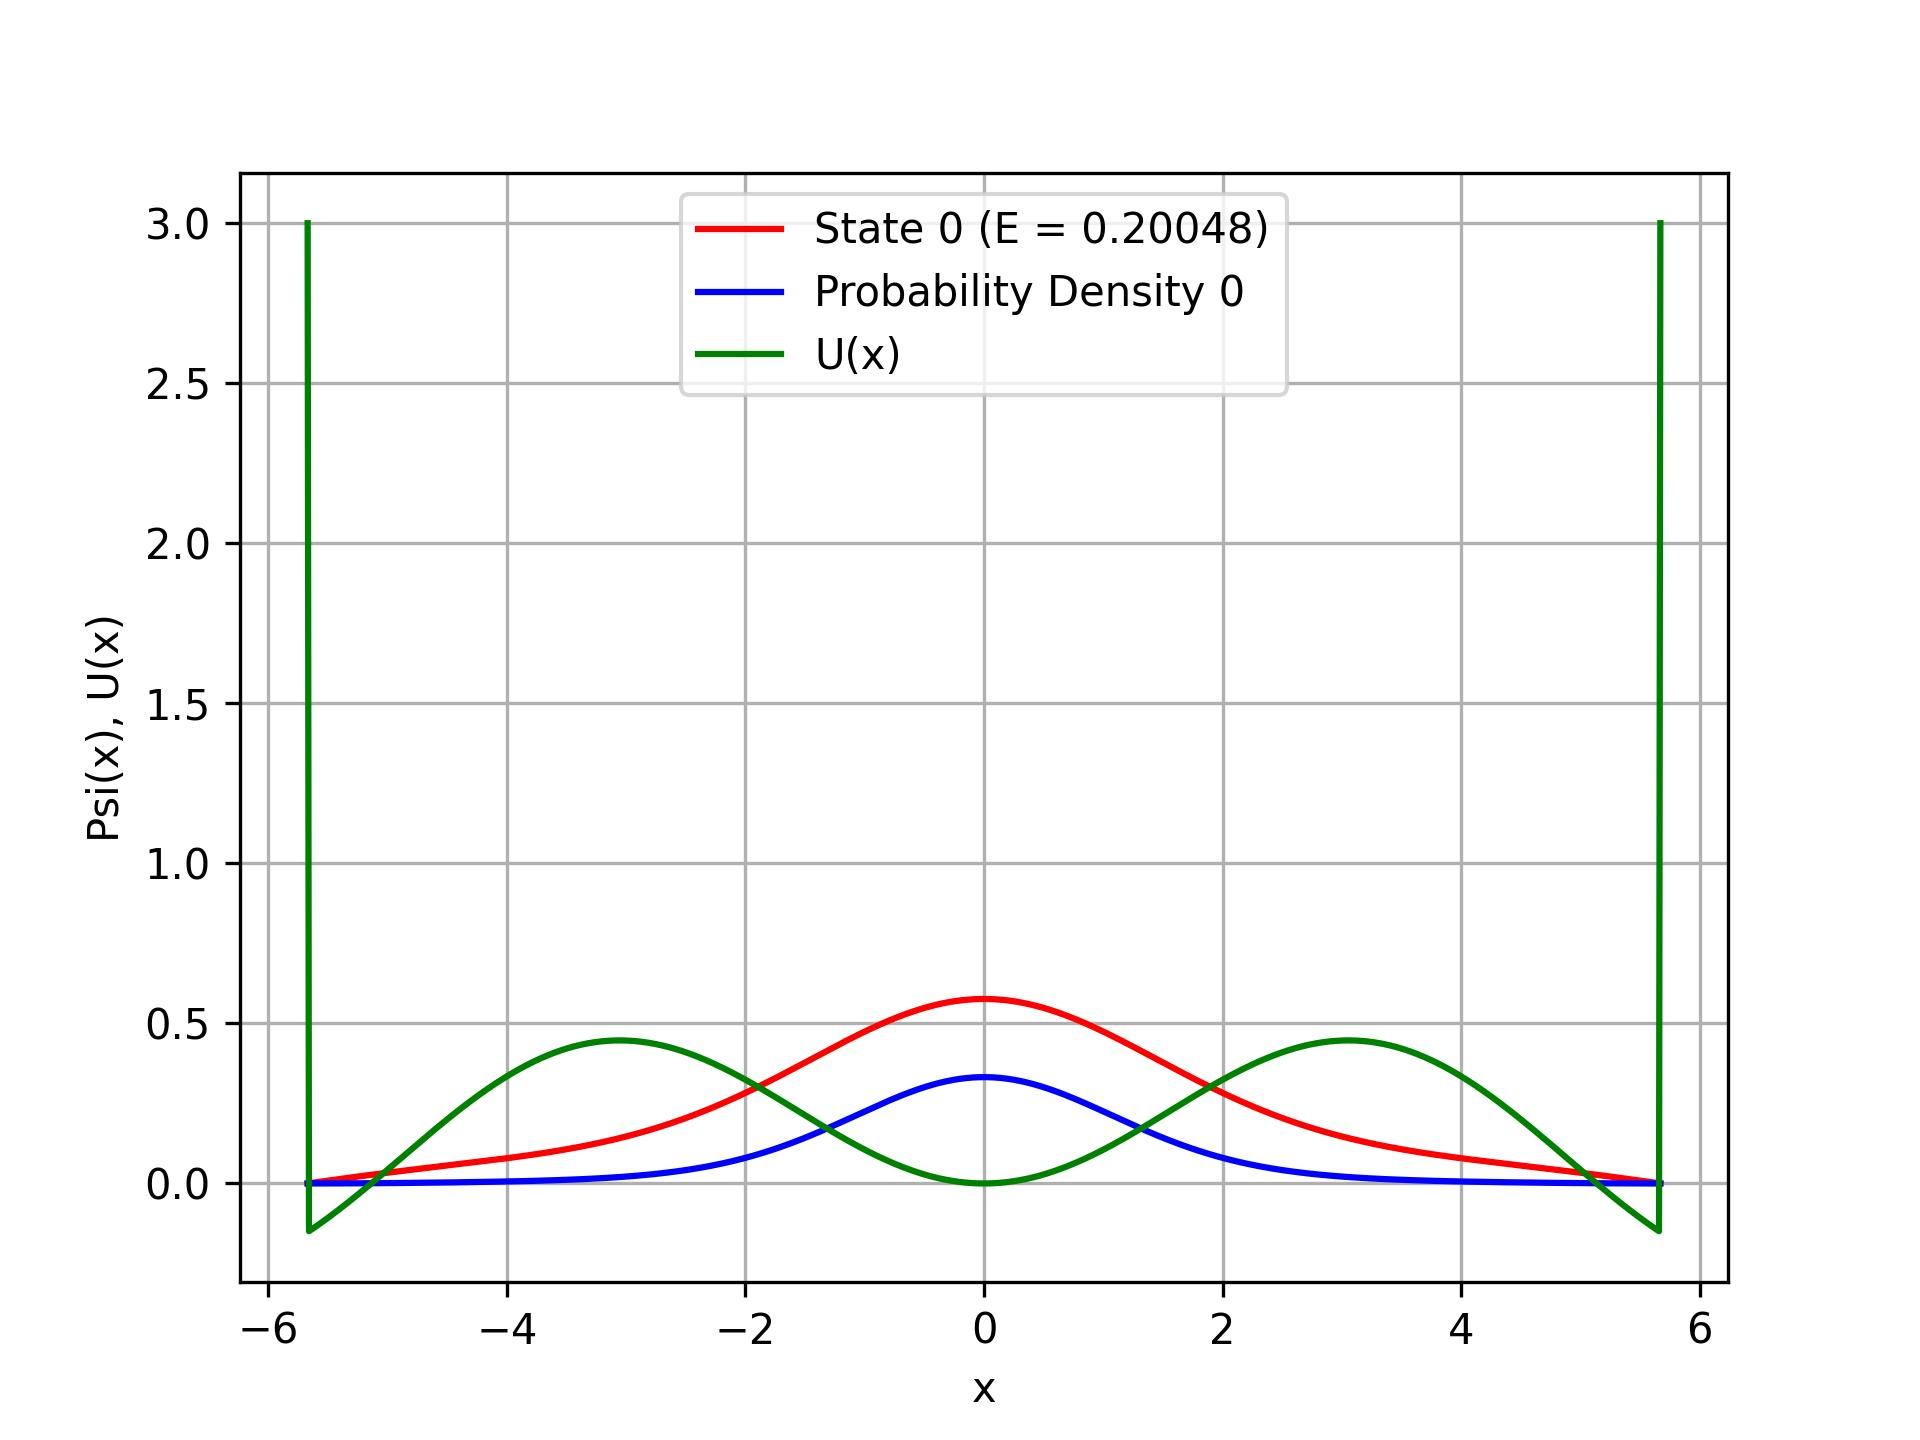
\includegraphics[width=0.6\linewidth]{State 0 probability density}
    \caption{Волновая функция основного состояния, полученная методом Ритца}\label{fig:State0PB}
\end{figure}

Волновая функция, полученная данным методом, согласно осцилляционной теореме соответствует основному состоянию.

Сравним волновые функции основного состояния, полученные методом Ритца и методом пристрелки (Рис.~\ref{fig:State0}):

\begin{figure}[h]
\centering
    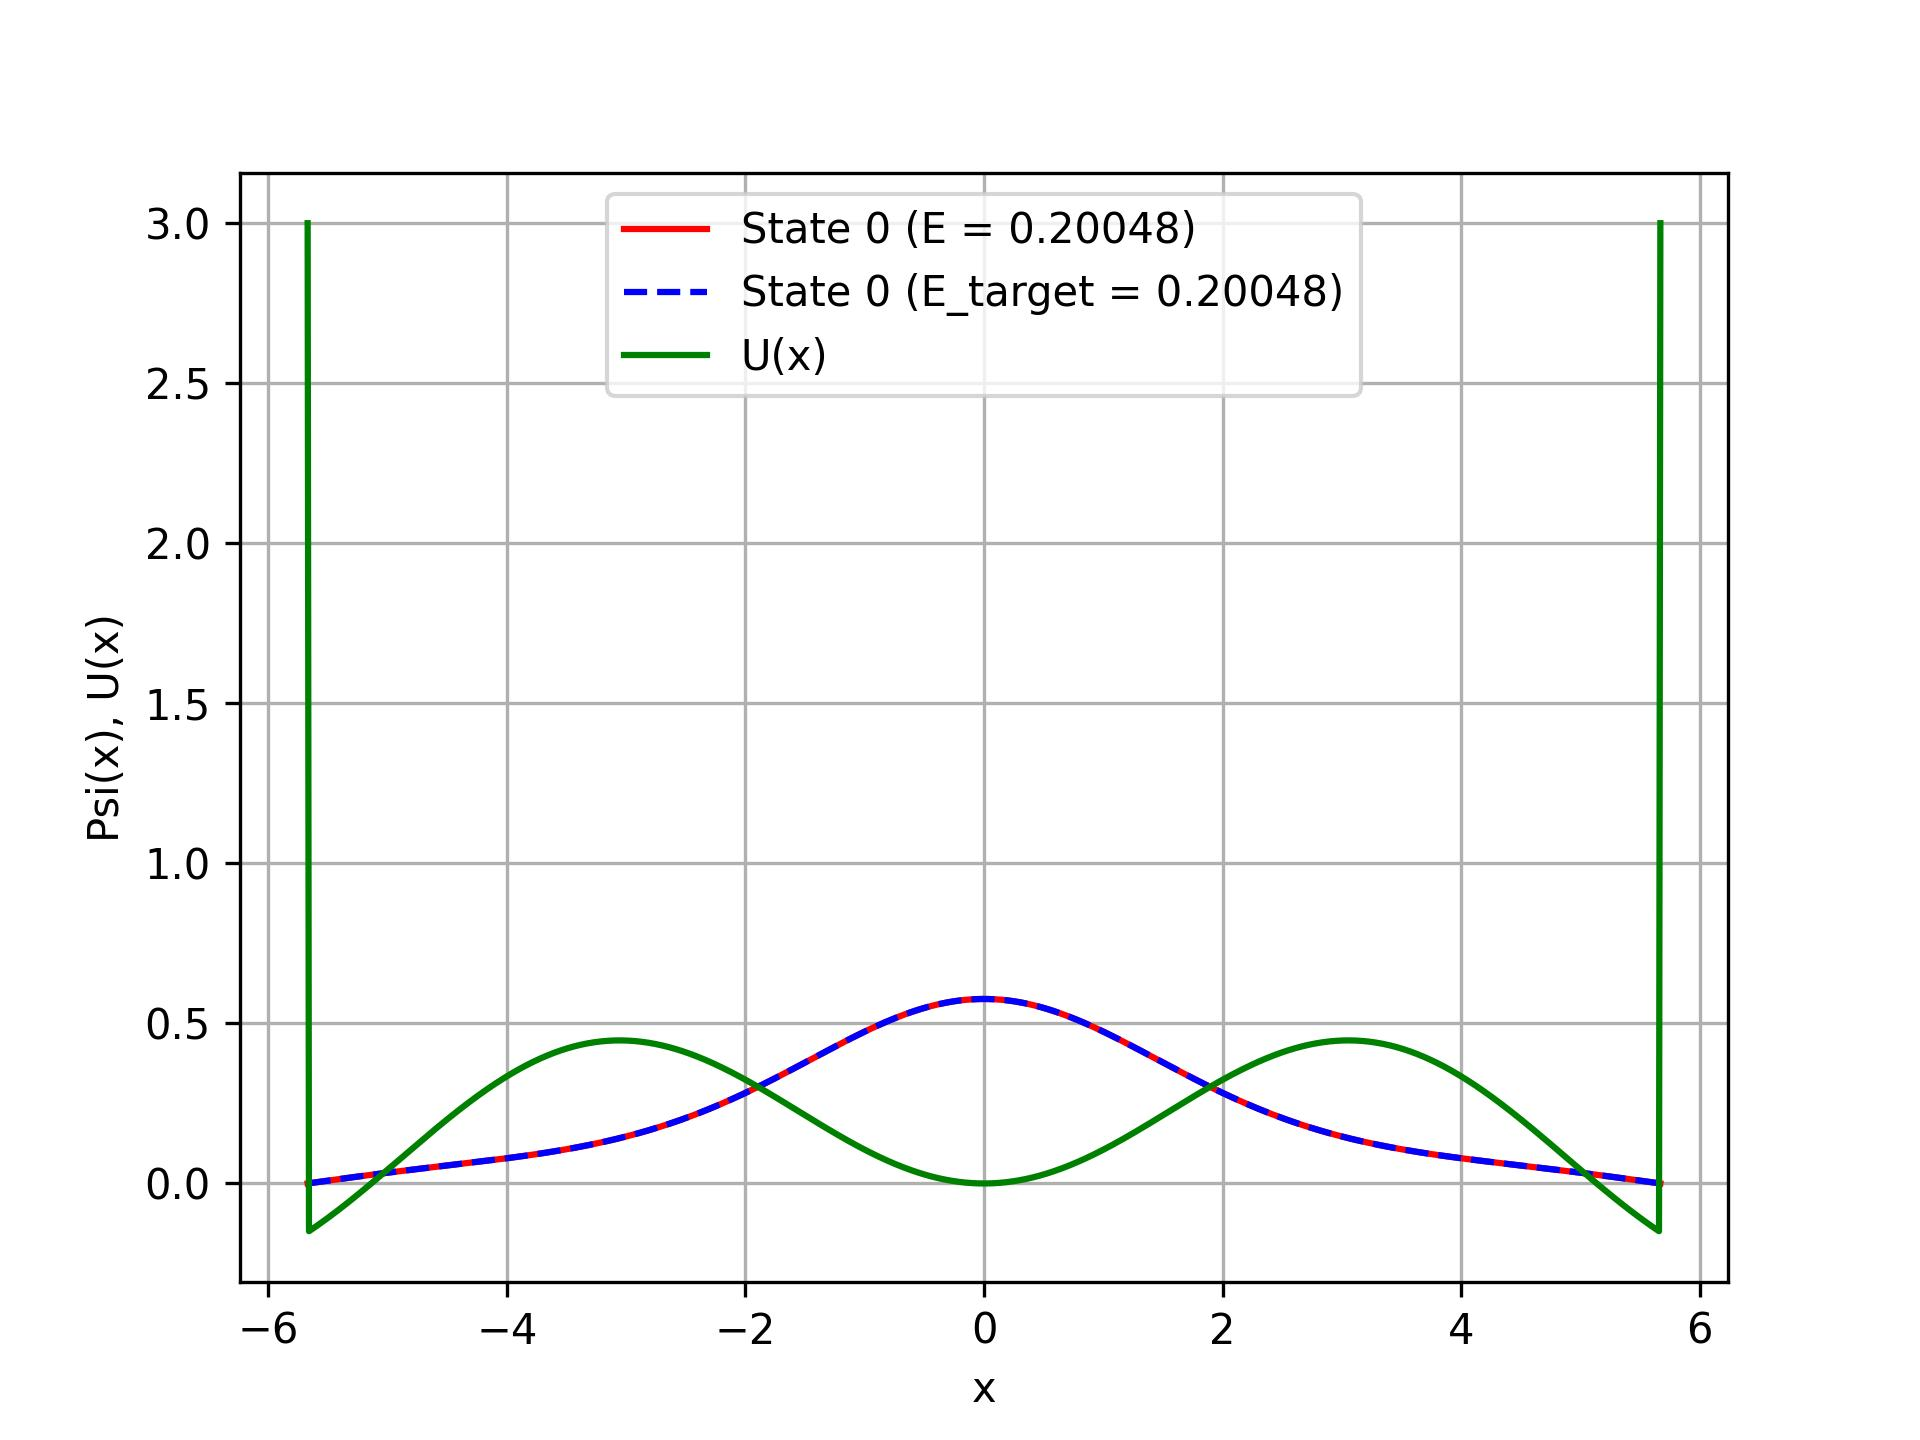
\includegraphics[width=0.6\linewidth]{State 0}
    \caption{Волновая функция основного состояния, сравнение методов}\label{fig:State0}
\end{figure}


Как можно заметить, данные функции не сходятся, даже более того - функция, полученная методом Ритца, имеет 0 пересечений с осью абсцисс,
в то время как функция, полученная методом пристрелки имеет два пересечения.
Как было рассмотрено в предыдущих лабораторных работах -- основным состоянием для заданной потенциальной функции является состояние с индексом $k=2$.
Предположим, что данный метод либо не подходит для решения текущей задачи (задача в которой основное состояние начинается с $k=2$).

Рассмотрим следующие состояния, полученные текущими методами.

\begin{figure}[H]
    \centering
    \begin{subfigure}{0.45\textwidth}
        \centering
        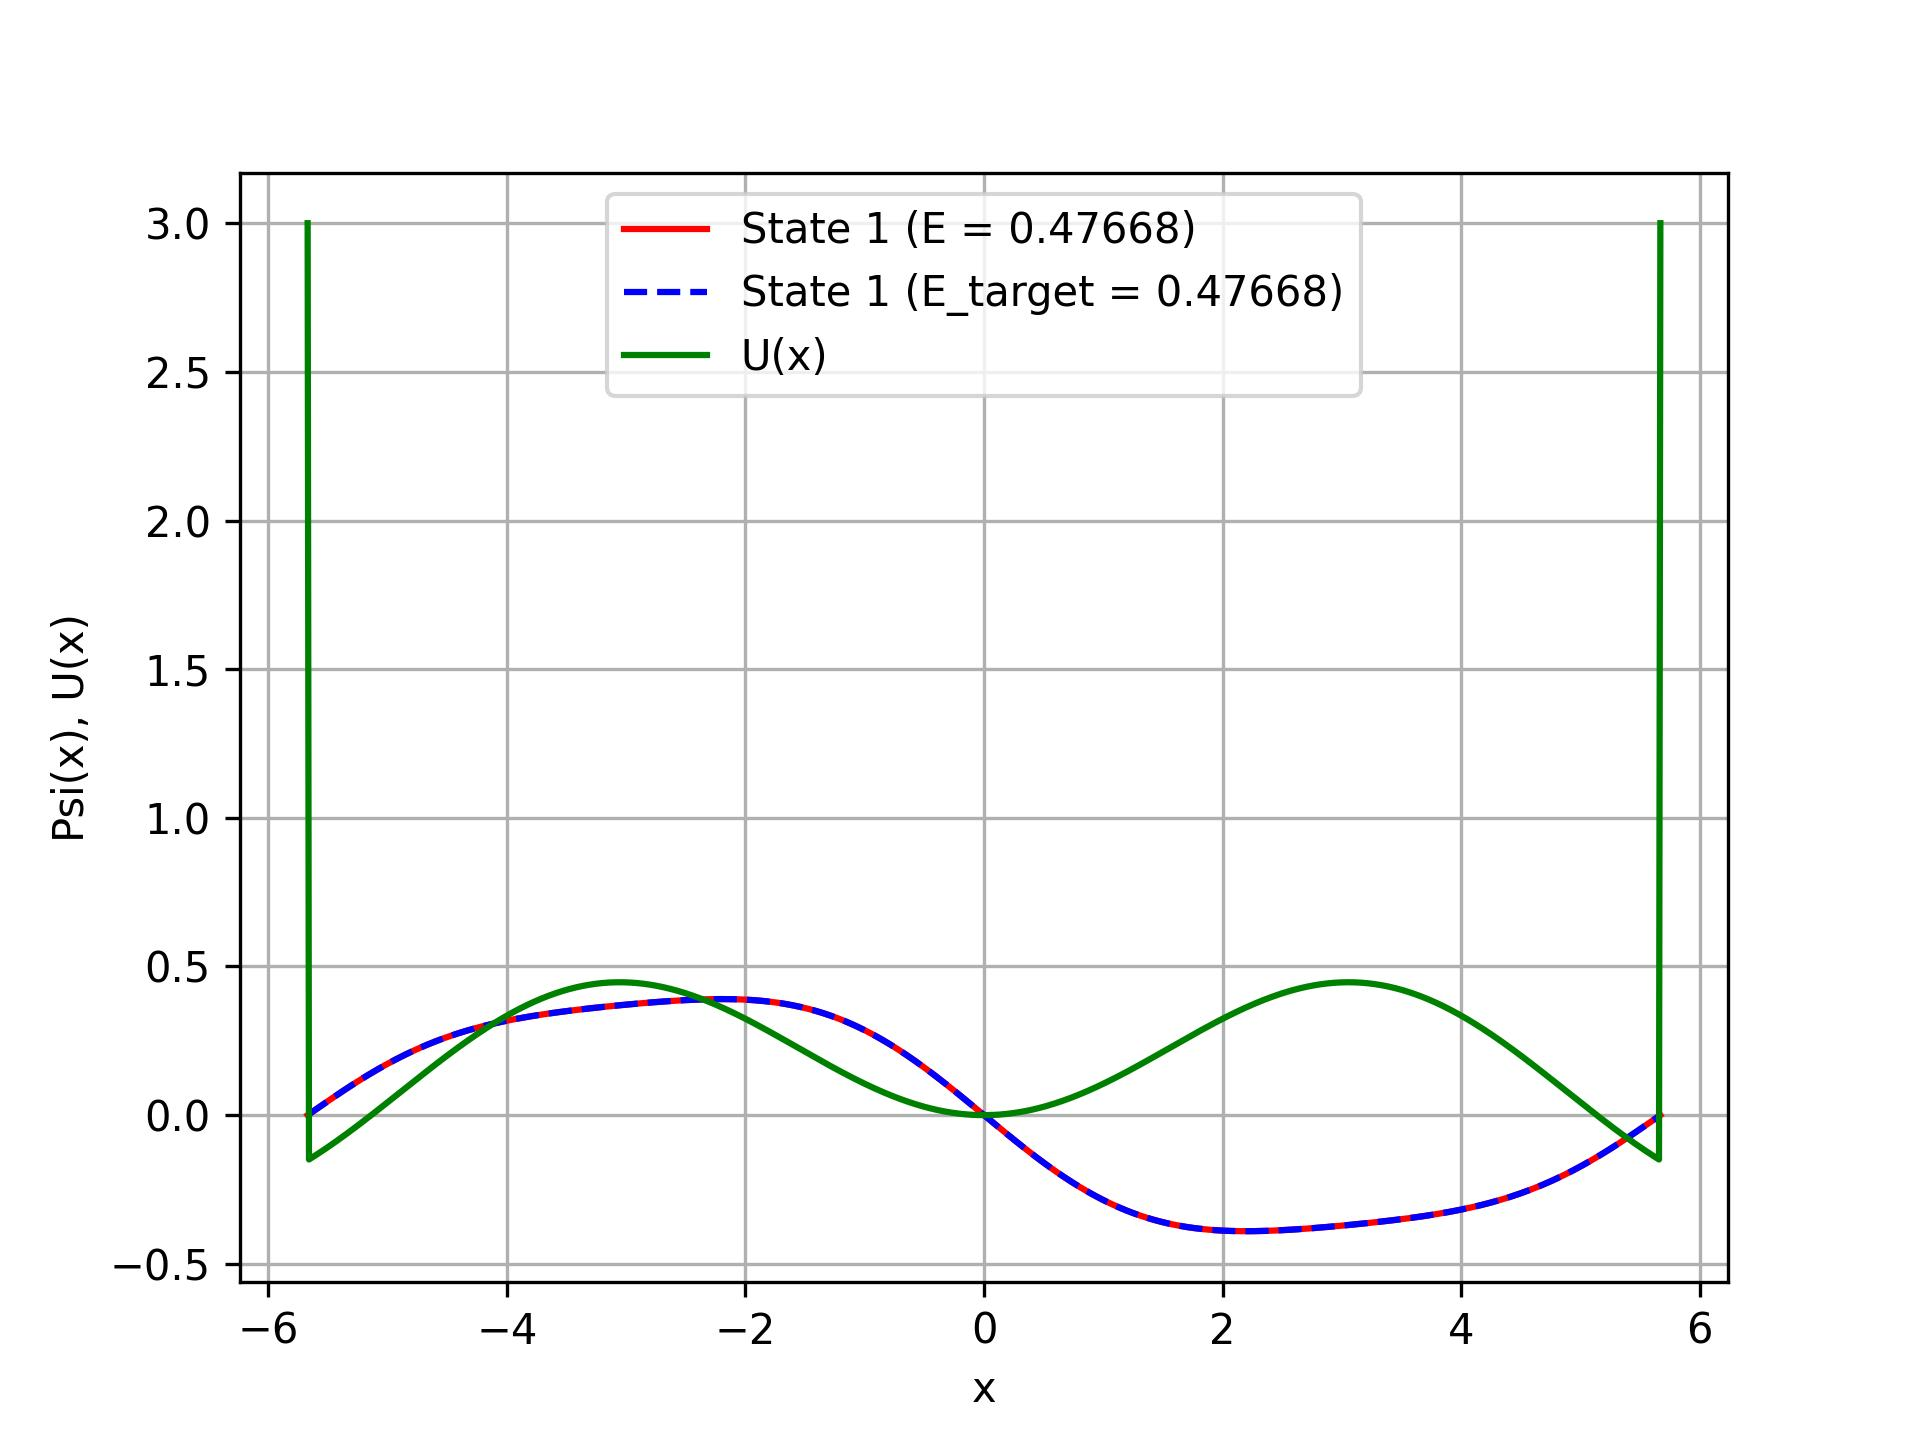
\includegraphics[width=0.9\linewidth]{State 1}
        \caption{Состояние 1}
        \label{fig:state1}
    \end{subfigure}%
    \begin{subfigure}{0.45\textwidth}
        \centering
        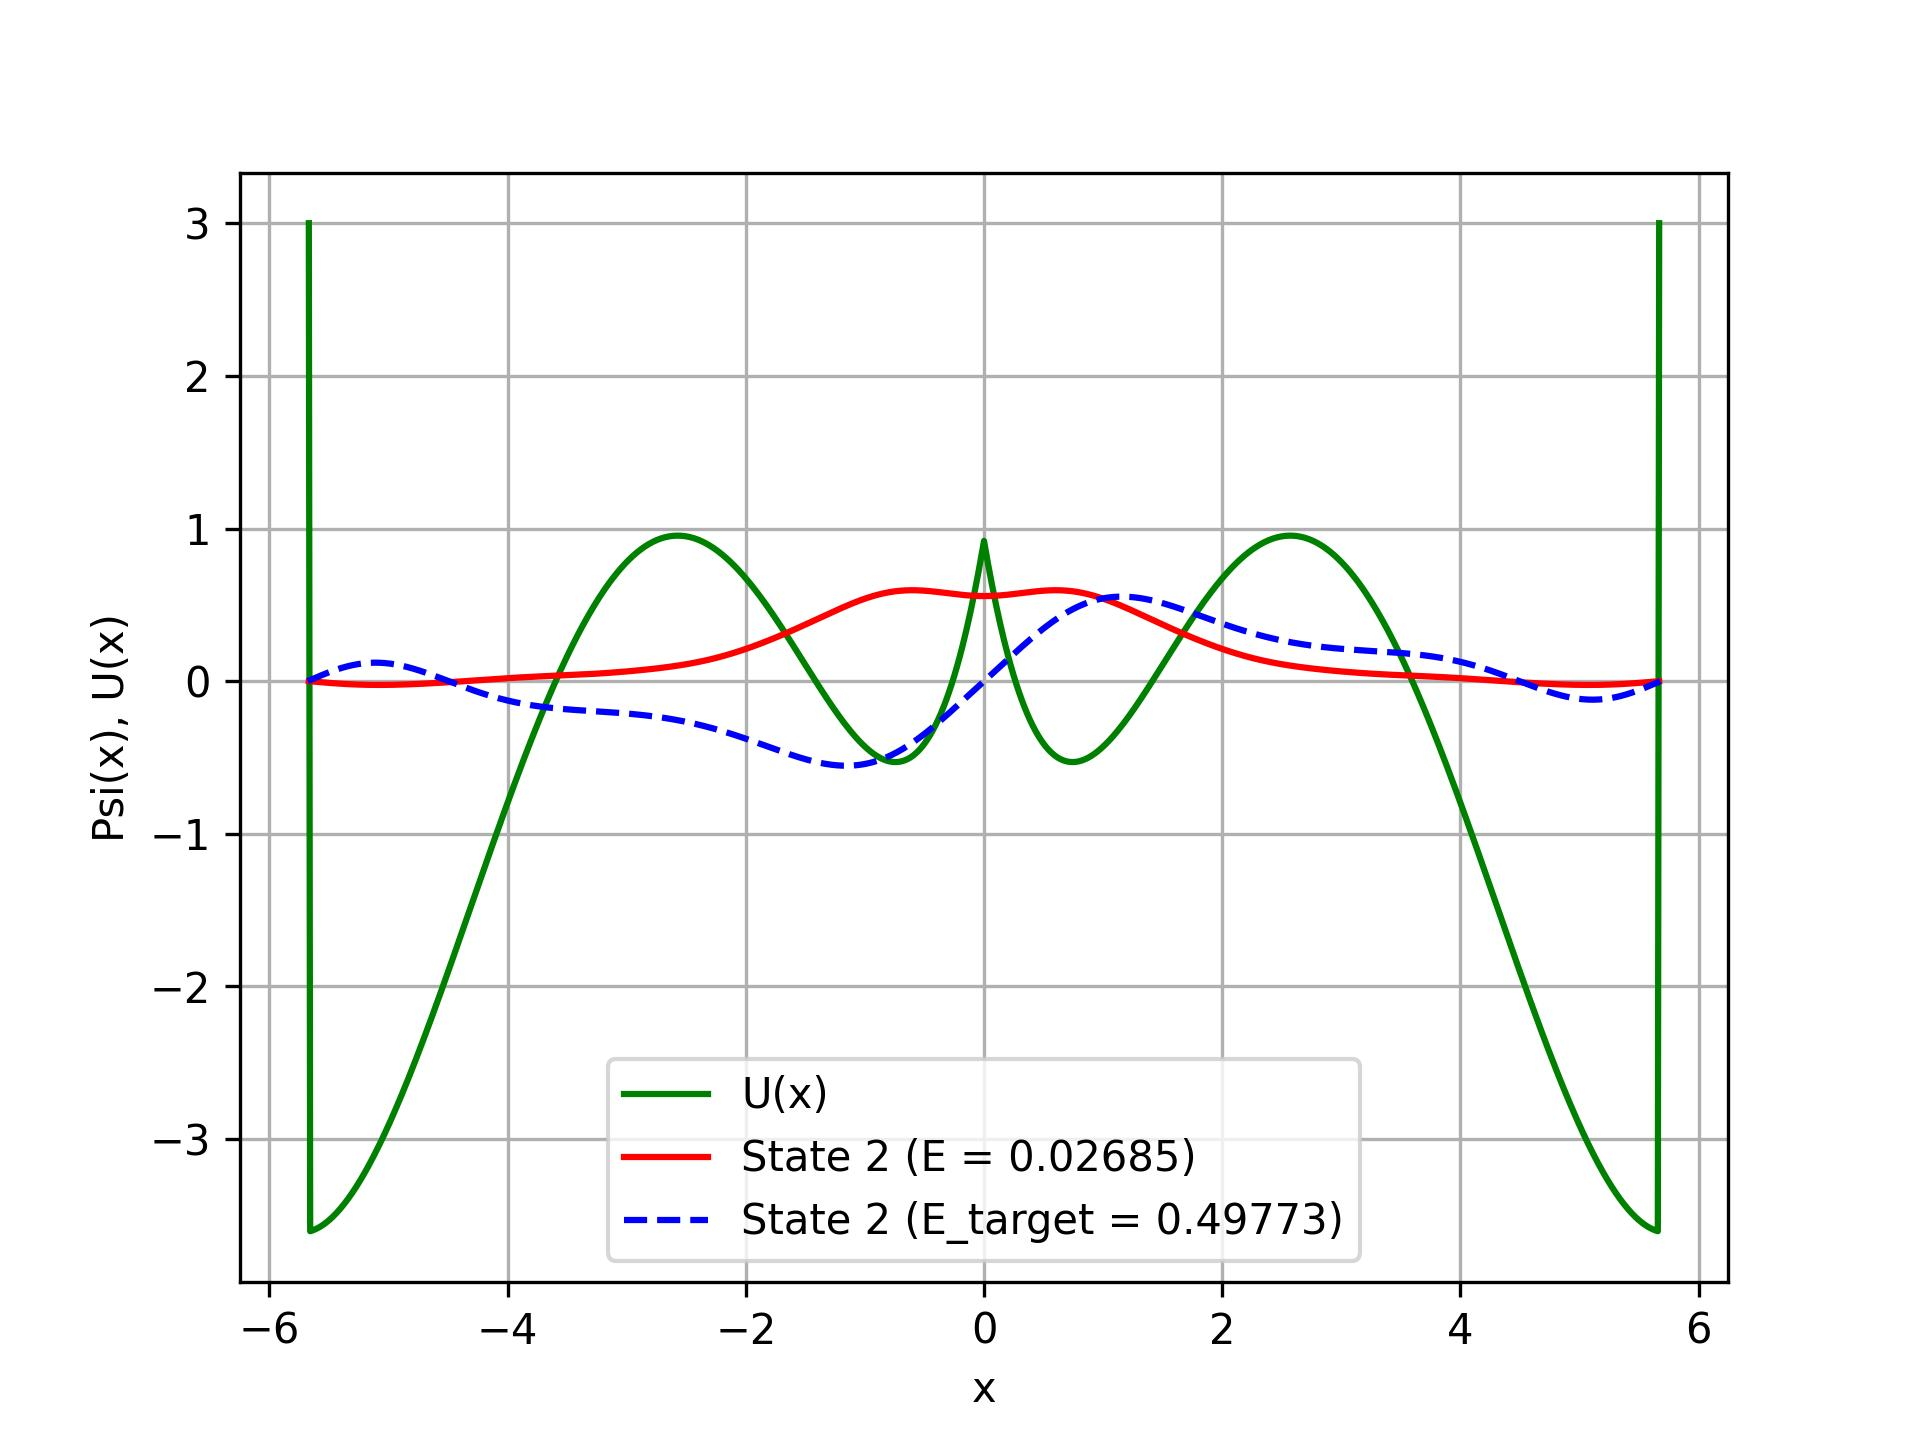
\includegraphics[width=0.9\linewidth]{State 2}
        \caption{Состояние 2}
        \label{fig:state2}
    \end{subfigure}%
\caption{Графики для состояний 1 и 2}
\end{figure}
\label{fig:state12}
Как можно заметить, в обоих случаях графики функций разнятся.
Сравним энергии, полученные в процессе решения задачи методом Ритца и методом пристрелки:
\begin{table}[H]
    \centering
    \noindent
    \begin{tabularx}{\linewidth}{|X|X|X|}
        \hline
        \textbf{Состояние}&\textbf{Метод Ритца энергия, а.е.}&\textbf{Метод пристрелки энергия, а.е.}\\
        \hline
        Основное & $-1.264468$ & $0.026429199218641876$\\
        \hline
        1-е возбужденное & $-1.264465$ & $0.49773486328114225$\\
        \hline
        2-е возбужденное & $0.026845$ & $0.8155639648436425$\\
        \hline
        3-е возбужденное & $0.498926$ & $0.9052211914061424$\\
        \hline
        4-е возбужденное & $0.828370$ & $2.0405639648435283$\\
        \hline
    \end{tabularx}\label{tab:energies}
\end{table}

Как можно заметить, энергии, полученные методом Ритца и методом пристрелки разнятся, однако,
также можно заметить что данные энергии сходятся, но для разных состояний.
Имеет смысл предположить что в силу большей точности метод Ритца позволяет найти значения энергий,
которые метод Пристрелки даст только с крайне малым шагом $\triangleE$,
при котором вычисления будут производиться значительно большое количество времени.

%Подытожив, выведем энергии полученные для первых двух состояний (включая основное) разными методами,
%а также квантовомеханические средние $\langle p(x) \rangle$ и $\langle p(x^2) \rangle$
%
%
%\noindent
%\begin{tabularx}{\linewidth}{|c|c|X|X|X|}
%    \hline
%    \textbf{Метод}&\textbf{Состояние}&\textbf{Энергия, а.е.}&\textbf{$\langle p(x) \rangle$}&\textbf{$\langle p(x^2) \rangle$} \\
%    \hline
%    Ритца & Основное & $-1.264468$ & $0.000000e+00$ & $3.070530e-01$ \\
%    \hline
%    Пристрелки & Основное & $-1.283224$ & $0.000000e+00$ & $3.070530e-01$ \\
%    \hline
%    Ритца & 1-е возбужденное & $0.815564$ & $0.000000e+00$ & $2.435363$ \\
%    \hline
%    Пристрелки & 1-е возбужденное & $0.815564$ & $0.000000e+00$ & $2.435363$ \\
%    \hline
%    Ритца & 2-е возбужденное & $0.815564$ & $0.000000e+00$ & $2.435363e+00$\\
%    \hline
%    Пристрелки & 2-е возбужденное & $0.815564$ & $0.000000e+00$ & $2.435363e+00$\\
%    \hline
%\end{tabularx}
\newpage

\section{Заключение}\label{sec:zakl}

Таким образом, было получено численное решение для задачи о частице в одномерной квантовой яме с бесконечными стенками при помощи метода Ритца.
Были получены значения энергий и волновые функции основного и второго возбужденного состояний.
Полученные волновые функции соответствуют осцилляционной теореме.
%Кроме того, для каждого состояния были вычисленные квантовомеханические средние~$\langle p(x) \rangle, \langle p(x^2) \rangle$.
В процессе выполнения задачи был также сделан вывод о точности метода Ритца - он позволяет находить б\'{о}льшее количество энергий чем метод пристрелки.
Как минимум, для текущего варианта задачи получилось найти значения энергий, которые не были получены при шаге $\triangle E = 0.001$ в методе пристрелки.


\newpage

\appendix

\section*{Приложение}\label{sec:extras}
\begin{lstlisting}[language=Python, caption=Код файла solver.py,label={lst:solver}]
import numpy as np
import matplotlib.pyplot as plt
from scipy.special import eval_laguerre

def draw_potential_graph():
    n = 500
    c_energy = 27.212
    c_length = 0.5292
    v0 = 25.0 / c_energy
    l = 3.0 / c_length
    a, b = -l, l
    x = np.linspace(a - 0.01, b + 0.01, n)

    def u_func():
        u_val = np.zeros(n)
        for i in range(n):
            if np.abs(x[i]) <= l:
                u_val[i] = v0 * eval_laguerre(5, np.abs(x[i]))
            else:
                u_val[i] = l

        return u_val

    y = u_func()

    plt.plot(x, y, 'g-', linewidth=6.0, label="U(x)")
    plt.title(f"Potential function graph")
    plt.xlabel("X")
    plt.ylabel("Y")
    plt.grid(True)
    plt.legend()

    plt.savefig('Potential_func_graph.jpg')
    plt.show()


class Solver:
    # Params
    def __init__(self):
        self.U_min = -0.149124
        self.c_energy = 27.212
        self.c_length = 0.5292
        self.V0 = 25.0 / self.c_energy
        self.L = 3.0 / self.c_length
        self.A, self.B = -self.L, self.L
        self.n = 650
        self.h = (self.B - self.A) / (self.n - 1)
        self.c, self.W = self.h ** 2 / 12.0, 3.0
        self.Psi, self.Fi, self.X = np.zeros(self.n), np.zeros(self.n), np.linspace(self.A, self.B, self.n)
        self.r = (self.n - 1) // 2 - 80
        self.limit_value = 4.0

        self.d1, self.d2 = 1.e-09, 1.e-09
        self.tol = 1e-6

        self.E_min, self.E_max, self.step = self.U_min + 0.01, 2.0, 0.01


    def u_func(self, x):
        # Check if x is a scalar
        if np.isscalar(x):
            # x - scalar
            return self.V0 * eval_laguerre(5, abs(x)) if abs(x) <= self.L else self.W
        u_val = np.zeros(self.n)
        for i in range(self.n):
            if np.abs(x[i]) <= self.L:
                u_val[i] = self.V0 * eval_laguerre(5, np.abs(x[i]))
            else:
                u_val[i] = self.L
        return u_val

    def q(self, e, x):
        return 2.0 * (e - self.u_func(x))


    @staticmethod
    def derivative_func(y, h, m):
        return (y[m - 2] - y[m + 2] + 8.0 * (y[m + 1] - y[m - 1])) / (12.0 * h)


    def normalize_wave_function(self, y):
        norm = np.sqrt(np.trapz(y ** 2, self.X))
        return y / norm


    @staticmethod
    def mean_momentum(psi, x):
        h_bar = 1.0
        d_psi_dx = np.gradient(psi, x)
        integrand = psi.conj() * d_psi_dx
        mean_px = -1j * h_bar * np.trapz(integrand, x)
        return mean_px.real


    @staticmethod
    def mean_square_momentum(psi, x):
        h_bar = 1.0
        d2_psi_dx2 = np.gradient(np.gradient(psi, x), x)
        integrand = psi.conj() * d2_psi_dx2
        mean_px2 = -h_bar**2 * np.trapz(integrand, x)
        return mean_px2.real

    def f_fun(self, e, n):
        f = np.array([self.c * self.q(e, self.X[i]) for i in np.arange(n)])
        self.Psi[0] = 0.0
        self.Fi[n - 1] = 0.0
        self.Psi[1] = self.d1
        self.Fi[n - 2] = self.d2

        for i in np.arange(1, n - 1, 1):
            p1 = 2.0 * (1.0 - 5.0 * f[i]) * self.Psi[i]
            p2 = (1.0 + f[i - 1]) * self.Psi[i - 1]
            self.Psi[i + 1] = (p1 - p2) / (1.0 + f[i + 1])

        for i in np.arange(n - 2, 0, -1):
            f1 = 2.0 * (1.0 - 5.0 * f[i]) * self.Fi[i]
            f2 = (1.0 + f[i + 1]) * self.Fi[i + 1]
            self.Fi[i - 1] = (f1 - f2) / (1.0 + f[i - 1])

        p1 = np.abs(self.Psi).max()
        p2 = np.abs(self.Psi).min()
        big = p1 if p1 > p2 else p2

        self.Psi[:] = self.Psi[:] / big

        coefficient = self.Psi[self.r] / self.Fi[self.r]
        self.Fi[:] = coefficient * self.Fi[:]

        return Solver.derivative_func(self.Psi, self.h, self.r) - Solver.derivative_func(self.Fi, self.h, self.r)

    def energy_scan(self, e_min, e_max, step):
        energies = []
        values = []
        e = e_min
        while e <= e_max:
            f_value = self.f_fun(e, self.n)
            energies.append(e)
            values.append(f_value)
            e += step
        return energies, values

    def find_exact_energies(self, e_min, e_max, step, tol):
        energies, values = self.energy_scan(e_min, e_max, step)
        exact_energies = []
        for i in range(1, len(values)):
            log1 = values[i] * values[i - 1] < 0.0
            log2 = np.abs(values[i] - values[i - 1]) < self.limit_value
            if log1 and log2:
                e1, e2 = energies[i - 1], energies[i]
                exact_energy = self.bisection_method(e1, e2, tol)
                self.f_fun(exact_energy, self.n)
                exact_energies.append(exact_energy)
        return exact_energies

    def bisection_method(self, e1, e2, tol):
        while abs(e2 - e1) > tol:
            e_mid = (e1 + e2) / 2.0
            f1, f2, f_mid = self.f_fun(e1, self.n), self.f_fun(e2, self.n), self.f_fun(e_mid, self.n)
            if f1 * f_mid < 0.0:
                e2 = e_mid
            else:
                e1 = e_mid
            if f2 * f_mid < 0.0:
                e1 = e_mid
            else:
                e2 = e_mid
        return (e1 + e2) / 2.0

    def plot_wave_functions(self, energies):
        for i, E in enumerate(energies):
            self.f_fun(E, self.n)
            psi_norm = self.normalize_wave_function(self.Psi.copy())
            fi_norm = self.normalize_wave_function(self.Fi.copy())
            mean_px = Solver.mean_momentum(fi_norm, self.X)
            mean_px2 = Solver.mean_square_momentum(fi_norm, self.X)
            file = open("result.txt", "w")
            file.close()
            file1 = open("result.txt", "a")
            print(f"Condition {i}: E = {E:.6f}, <p_x> = {mean_px:.6e}, <p_x^2> = {mean_px2:.6e}")
            print(f"Condition {i}: E = {E:.6f}, <p_x> = {mean_px:.6e}, <p_x^2> = {mean_px2:.6e}", file = file1)

            plt.scatter(self.X[self.r], psi_norm[self.r], color='red', s=50, zorder=5)  # Point at Psi
            plt.scatter(self.X[self.r], fi_norm[self.r], color='blue', s=50, zorder=5)  # Point at Fi
            plt.plot(self.X, [self.u_func(x) for x in self.X], 'g-', linewidth=6.0, label="U(x)")
            plt.plot(self.X, psi_norm, label=f"Normalized condition Psi {i}")
            plt.plot(self.X, fi_norm, '--', label=f"Normalized condition Phi {i}")
            plt.title(f"Condition {i} (Normalized) for E = {E:.4f}")
            plt.xlabel("X")
            plt.ylabel("Normalized wave functions")
            plt.grid(True)
            plt.legend()
            plt.savefig(f"Condition_{i}_(normalized).jpg", dpi=300)
            plt.show()


            prob_density_psi = psi_norm**2
            prob_density_fi = fi_norm**2
            plt.plot(self.X, [self.u_func(x) for x in self.X], 'g-', linewidth=6.0, label="U(x)")
            plt.plot(self.X, prob_density_psi, label=f"Probability density Psi condition {i+1}")
            plt.plot(self.X, prob_density_fi, '--', label=f"Probability Density Phi condition {i+1}")
            plt.title(f"Condition {i} - Probability density where E = {E:.4f}")
            plt.xlabel("X")
            plt.ylabel("Probability density")
            plt.grid(True)
            plt.legend()
            plt.savefig(f"Condition_{i}_(Probability_density).jpg", dpi=300)
            plt.show()


    def solve(self):
        e_min, e_max, step = self.U_min + 0.01, 3.0, 0.01
        exact_energies = self.find_exact_energies(e_min, e_max, step, self.tol)

        if len(exact_energies) == 0:
            print("Error: energies were not found.")
        else:
            print("Energies:")
            for i, E in enumerate(exact_energies):
                print(f"Condition {i}: Energy = {E:.6f}")

            self.plot_wave_functions(exact_energies)
\end{lstlisting}


\newpage
\begin{thebibliography}{9}
\bibitem{tim_shrod} Тимошенко Ю.К. \textit{Численное решение стационарного уравнения Шрёдингера.} Воронеж, 2019. 35 с.
\bibitem{python} Доля П.Г. \textit{Введение в научный Python} Харьков: ХНУ, 2016. 265 с.
\bibitem{dav} Давыдов А.С. \textit{Квантовая механика} СПб: БХВ-Петербург, 2011. 704 с.
\bibitem{tim_lectures} Тимошенко Ю.К. \textit{Лекционный материал} 2019.
\end{thebibliography}


\end{document}